This module encapsulate all the knowledge needed by the agent to make decisions. This module is divided in specialized sub-modules, which are in charge to have the information specific information and make inference from these. These sub-modules are:
\begin{itemize}
	\item \textit{Sensory information and processing}: sense the robot's environment. Depending of the capabilities of the robotic platform, this module could capture meaningful information.
	\item \textit{World model}: is the representation of the surround environment.
	\item \textit{Social world model}: infers the current situation, and it has a the possible emotional state of the other people that are present.
	\item \textit{Rational social model}: has the relation of the character with other people and roles.
	\item \textit{Emotional model}: infers the emotional state based on the information coming from the social world model and rational social model.
	\item \textit{Delegated goals}: are those responsibilities that the agent have in order to perform its part on a play.
\end{itemize}
\subsection{The delegated goals}
The delegated goals are an important component for a robo-actor because encapsulates his functional purpose of acting. the whole structure and behavior of a play described in the script is represented as a knowledge in the agent. More specifically, this knowledge of a play is represented as a delegated goals, which is nothing more than an structured way that supports the motivation handler. 

This information is encapsulated in the script. Then, each line in the script artifact gives information about the current situation and emotional states of others. The current situation, consist of two kind of knowledge. 

\begin{itemize}
\item First, the space information. It encapsulate every object and person relative position in scene each time. 

\item Second, the social information. It encapsulates emotions and mental states from others in scene.
\end{itemize}

For each kind of information exist an ontology that defines the terms and meaning of each piece of information. Both ontologies are common to all agent. Then, they are designed for the entire multi-agent system.  

In the other hand, notice that the information described in each delegated goal doesn't have to be complete. It is represented only what matters at this moment, so the play will be well developed.

The delegated goals are given by the script and the information can represent as a double linked list in which each node becomes a goal. This goal encapsulates knowledge for a specific situation in scene  (see Figure  \ref{fig:ScriptRepresentation}).

\begin{figure}
	\centering
	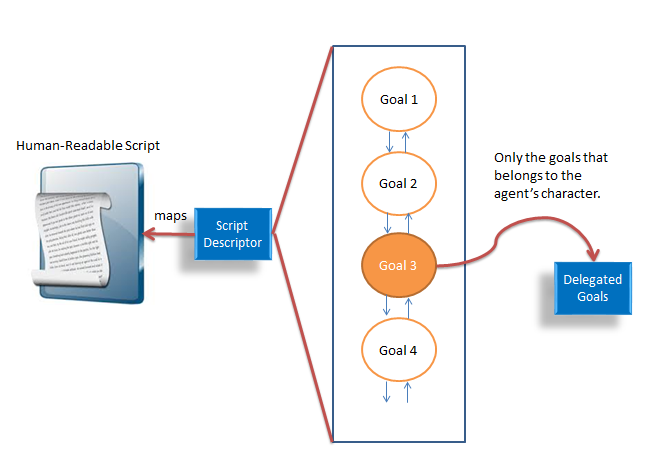
\includegraphics[width=0.5\textwidth]{Images/ScriptRepresentation.png} 
	\caption{The script representation try to map the real script human-readable in terms that the agent could interpret as knowledge.}
	\label{fig:ScriptRepresentation}
\end{figure}


Therefore, the structure of one delegated goal is define as follows:
\begin{itemize}

\item The owner: Is the character or group of characters for which this goal is delegated.

\item The performative: which is the dialog of the owner. This performative is optional, because the dialog is not required in all cases in theatre context.

\item The pre-condition: indicates the facts that must be true for consider the goal as a potential goal to become a desire.

\item The post-condition: is the desire state of the world, it means those facts that the agent want to be true.

A fact is a true predicate (at least, true for the agent) about the world, this includes both social and space information. For example, a fact about space: "there is a table". This fact provides information about the existence of a object in scene. If is necessary more accurate information about a space fact, it could be indicated adding in which stage division the object is or adding spacial relationships like "the chair is to the right of the table". In the other hand, social information can be "Anna coughing and angry". In this case could be specified an action or an emotion about any other character.

\item The plan of action: is a predefined graph of simple actions that trace the path the agent have to follow in order to reach the goal's post-condition. With the graph representation the actions could be executed in parallel. This plan is covered with more detail in Motivation Section.
\end{itemize}
This structure maps the information about the play contained in a regular script, adding information and structured in a way that the robot can interpret and perform.  
